\documentclass[a4paper,12pt]{article}
\usepackage{graphicx}       %LaTeX package to import graphics

\usepackage[T1]{fontenc}
\usepackage[italian]{babel}

\usepackage{subcaption}

\usepackage{hyphenat}
\usepackage{array}
\usepackage{booktabs}       % Per linee orizzontali migliori
\usepackage{caption}        % Per personalizzare le didascalie<
\usepackage{multirow}       % Per combinare celle nelle colonne
\usepackage{float}
\usepackage{hyperref}

\usepackage{bm} 

\usepackage{amsmath}        % Per migliorare l'aspetto delle formule

\usepackage{todonotes}      % mettere le note dentro il documento

\usepackage{siunitx}        % Per formattare le unità di misura
\usepackage{gensymb}        % Simboli come °
\usepackage{xfrac}          % per fare le frazioni inclinate

\usepackage{pdfpages}

\usepackage{import}
\usepackage{frontespizio}

\usepackage{placeins}       %per non far andare le immagini al di fuori delle sezioni utilizzare il comando: \FloatBarrier non far superare le immagini quel punto

\usepackage{adjustbox}      % per dimensionare le immagini in modo automatico


\begin{document}

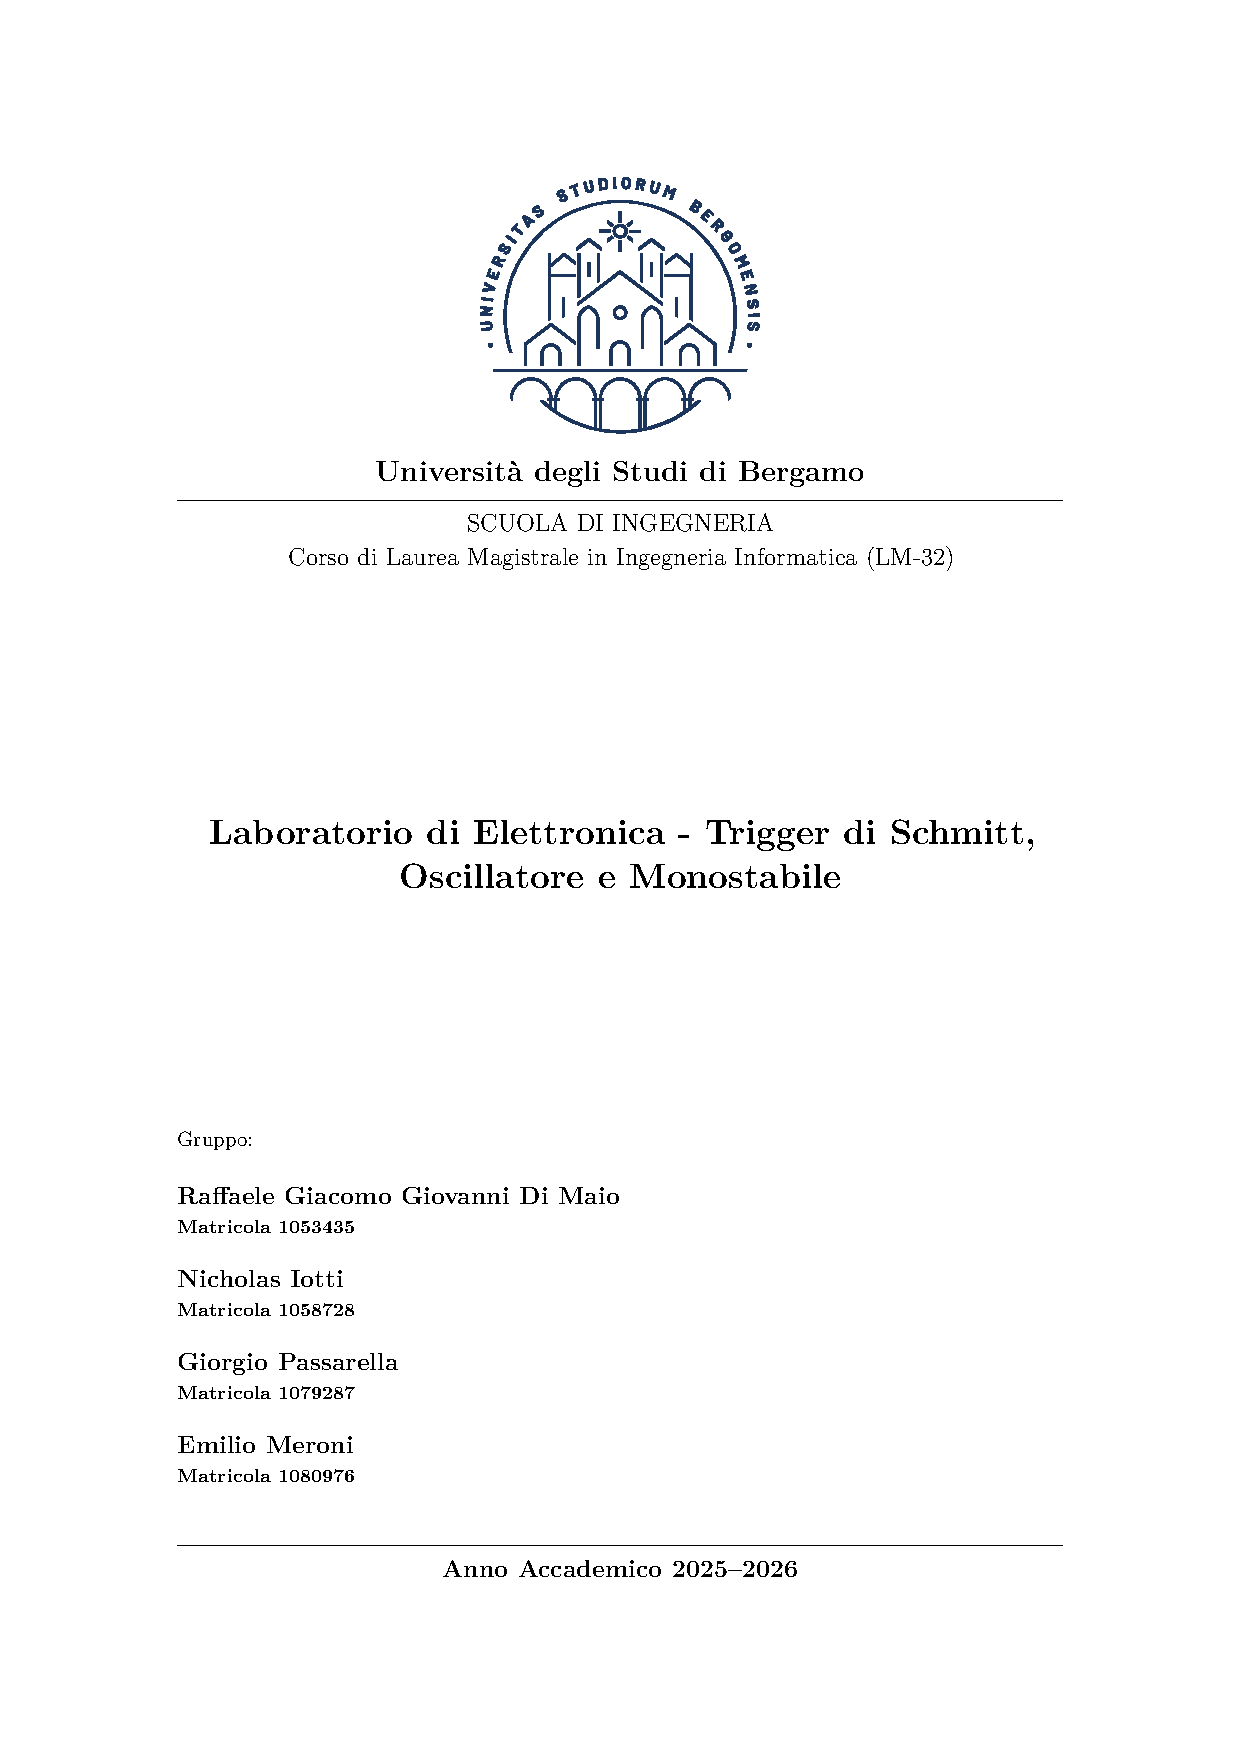
\includepdf{./frontespizio/frontespizio.pdf}

\section*{Trigger di Schmitt} 
L'amplificatore operazionale è un circuito elettronico che permette di confrontare due tensioni in ingresso e fornirne la differenza tra le due moltiplicata per un fattore di amplificazione $A$.
\begin{align*}
    V_{out} = A \cdot (V^+ - V^-)
\end{align*} 
Nel caso ideale $ A \rightarrow \infty $, pertanto l'uscita $V_{out}$ saturerà alla tensione di alimentazione positiva $V_{DD}$ solo se la differenza tra le due tensioni è maggiore di zero, altrimenti $V_{out} = -V_{DD}$.

Questo permette di utilizzarlo come comparatore di due tensioni. Tuttavia nella realtà sono presente delle problematiche dovute alla presenza di rumore elettronico che porta il segnale in uscita ad avere degli scatti spuri dovuti al ripetuto passaggio della soglia a causa del rumore stesso.
Per risolvere questo problema si utilizza il trigger di Schmitt \ref{fig:trigger_schmitt}.

\begin{figure}[h]
    \centering
    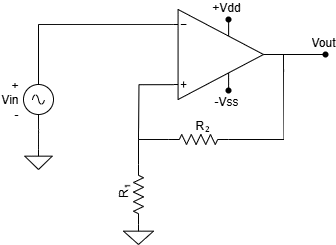
\includegraphics[width = 0.4\linewidth]{./immagini/schmitt/circuito.png}
    \caption{Schematico del Trigger di Schmitt}
    \label{fig:trigger_schmitt}
\end{figure}

Grazie all'utilizzo di una soglia dinamica, dipendente da $V_{out}$, permette di avere in uscita un segnale meno sensibile al rumore in ingresso.
\begin{enumerate}
    \item Ipotizzando uno stato iniziale in cui $V_{in} \ll 0$ allora si ha che $V_{out}$ satura a $V_{DD}$, questo porta ad avere un potenziale in:
    \begin{align*}
        V^+ = \frac{R_1}{R_2 + R_1} \cdot V_{DD} = \frac{V_{DD}}{2} = V^+_H
    \end{align*}
    determinando la soglia;
    \item Quando $V_{in} > V^+_H$ allora $V_{out} = V_{SS}$, ciò comporta ad avere $V^+ = \frac{V_{SS}}{2} = V^+_L$, ovvero una nuova soglia;
    \item Si rimane nello stato $2$ fino a quando $V_{in}$ diventa inferiore di $V^+_L$ ripartendo dal punto $1$.  
\end{enumerate} 

Questo andamento genera un ciclo di isteresi, figura \ref{fig:schmitt_mod_xy}, con ampiezza:
\begin{align*}
    \frac{2R_1}{R1+R2} \cdot V_{DD}
\end{align*}

\begin{figure}[h]
    \centering
    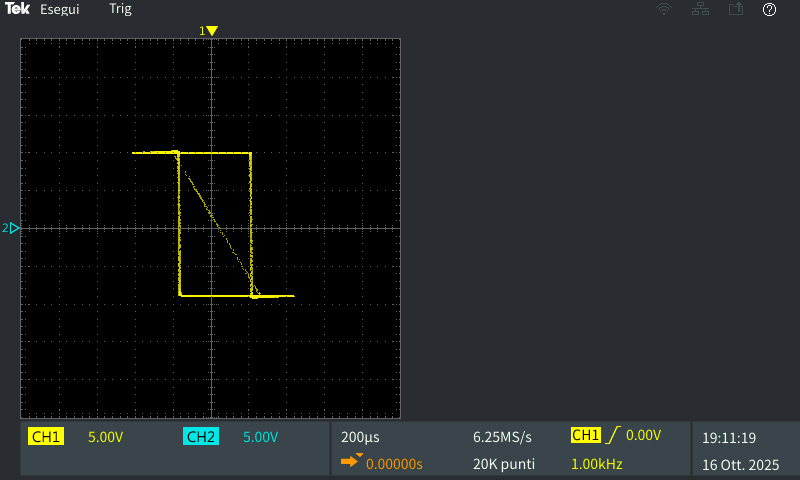
\includegraphics[width = 0.6\linewidth]{immagini/schmitt/schmitt_vin_vout_xy.png}
    \caption{Ciclo di isteresi del Trigger di Schmitt}
    \label{fig:schmitt_mod_xy}
\end{figure}

I valori utilizzati per testarne il funzionamento sono riportati a tabella \ref{tab:valori_trigger_schmitt}:
\begin{table}[h]
    \centering
    \setlength{\tabcolsep}{20pt}
    \begin{tabular}{c c}
        \toprule
        Elemento        & Valore            \\
        \midrule
        $V_{DD}$        & $10\,\mathrm{V}$  \\
        $V_{in\,pp}$    & $20\,\mathrm{V}$  \\
        $freq$             & $1\,\mathrm{KHz}$ \\
        $R_1$           & $9.0\,K\Omega$      \\
        $R_2$           & $9.0\,K\Omega$      \\
        \bottomrule
    \end{tabular}
    \caption{Valori utilizzati nel circutio: Trigger di Schmitt.}
    \label{tab:valori_trigger_schmitt}
\end{table}

Da cui sono stati ricavati i grafici a figura \ref{fig:schmitt_oscilloscopio}.


\begin{figure}[h]
    \centering
    \begin{subfigure}{0.49\linewidth}
        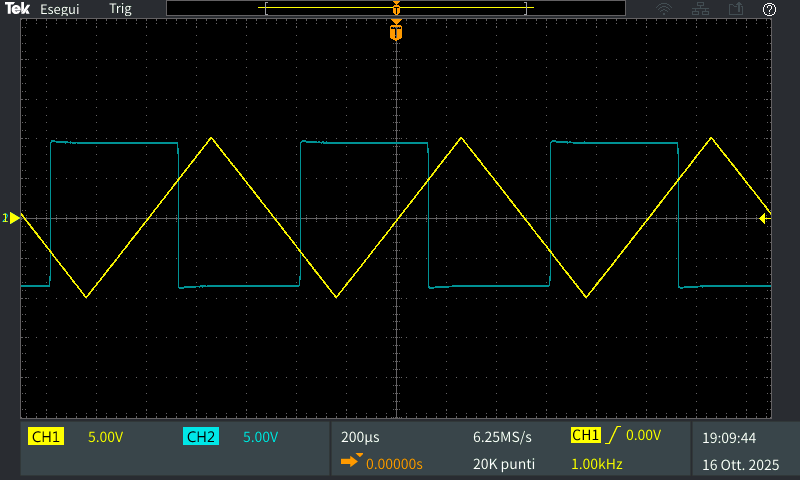
\includegraphics[width = \linewidth]{immagini/schmitt/schmitt_vin_vout.png}
        \caption{}
    \end{subfigure}
    \begin{subfigure}{0.49\linewidth}
        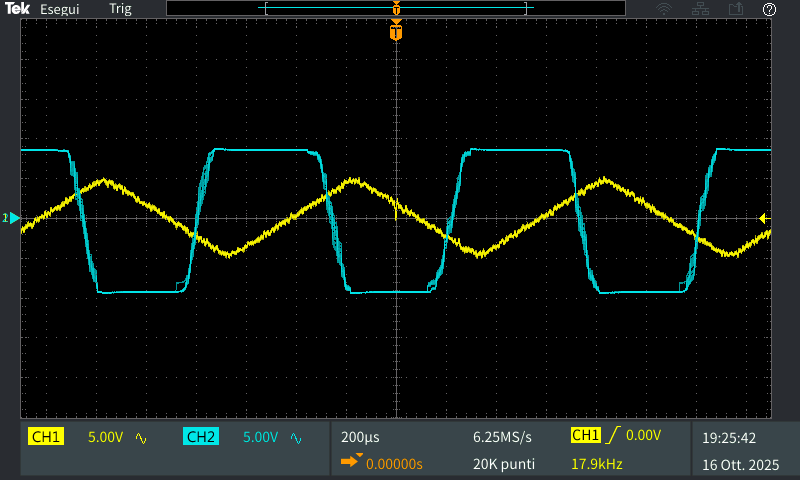
\includegraphics[width = \linewidth]{immagini/schmitt/schmitt_vin_vout_rumoroso.png}
        \caption{}
    \end{subfigure}
    \\[0.5cm]
    \begin{subfigure}{0.49\linewidth}
        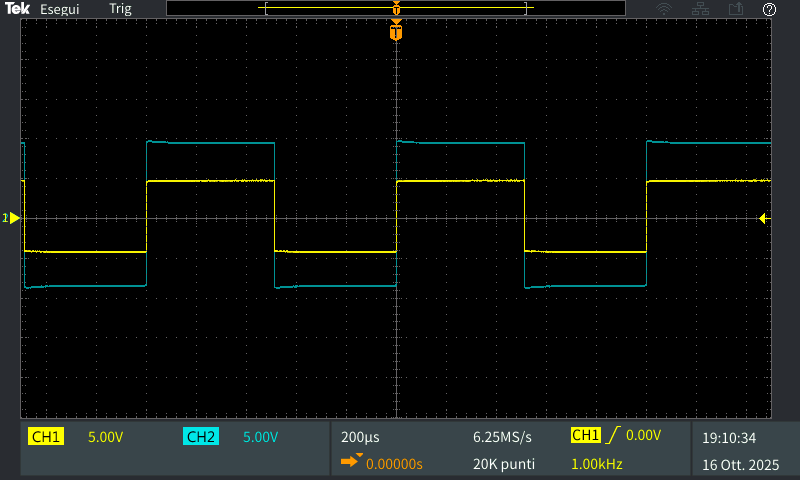
\includegraphics[width = \linewidth]{immagini/schmitt/schmitt_v+_vout.png}
        \caption{}
    \end{subfigure}
    \begin{subfigure}{0.49\linewidth}
        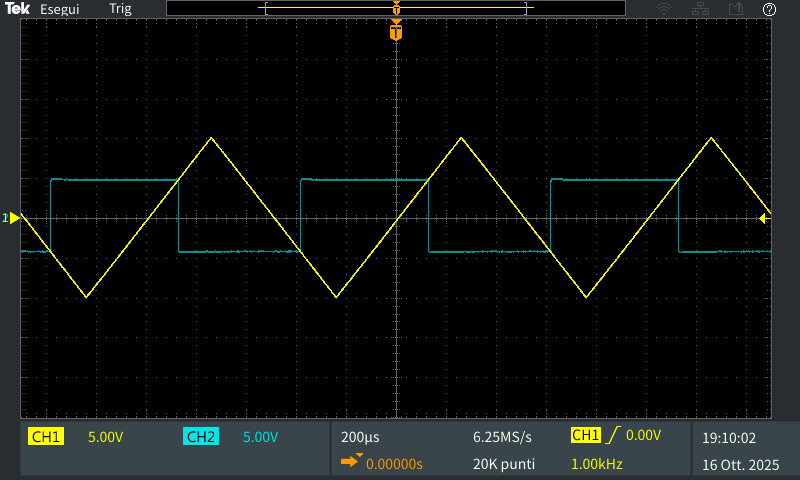
\includegraphics[width = \linewidth]{immagini/schmitt/schmitt_vin_v+.png}
        \caption{}
    \end{subfigure}
    \caption{Figure \textit{a} e \textit{b}: $V_{in}$ in giallo e $V_{out}$ in azzurro, confronto con segnale in ingresso non rumoroso (\textit{a}) e rumoroso (\textit{b}).
                Figura \textit{c}: in giallo la soglia dinamica, $V^+$, in azzurro l'uscita.
                Figura \textit{d}: Soglia dinamica confrontata con l'ingresso (in giallo).}
    \label{fig:schmitt_oscilloscopio}
\end{figure}


\section*{Oscillatore}
L'oscillatore è un circuito elettronico che genera un segnale ad onda quadra con un duty cycle pari al 50 per cento. Questo viene fatto attraverso la carica e la scarica di un condensatore (vedi circuito).
Il funzionamento del circuito si può suddividere in due fasi:
vout=Vdd
vout=-Vdd

E' possibile inoltre osservare la carica e scarica del condensatore nel tempo attraverso le seguenti equazioni:
Vc(t1)
Vc(t2)

Dalle quali possiamo ricavarci i due periodi T1, T2 e il periodo totale del segnale T:
T1=
T2=
T=

Infine modificando il valore della resistenza R si può controllare il valore della costante di tempo tau influenza la frequenza dell'onda generata (guardare plot) 

\begin{figure}[h]
    \centering
    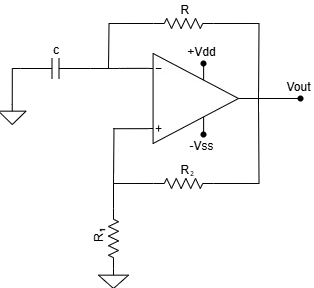
\includegraphics[width=0.4\linewidth]{immagini/ocillatore/circuito.png}
    \caption{Schematico oscillatore.}
    \label{fig:schematico_oscillatore}
\end{figure}

\begin{figure}[h]
    \centering
    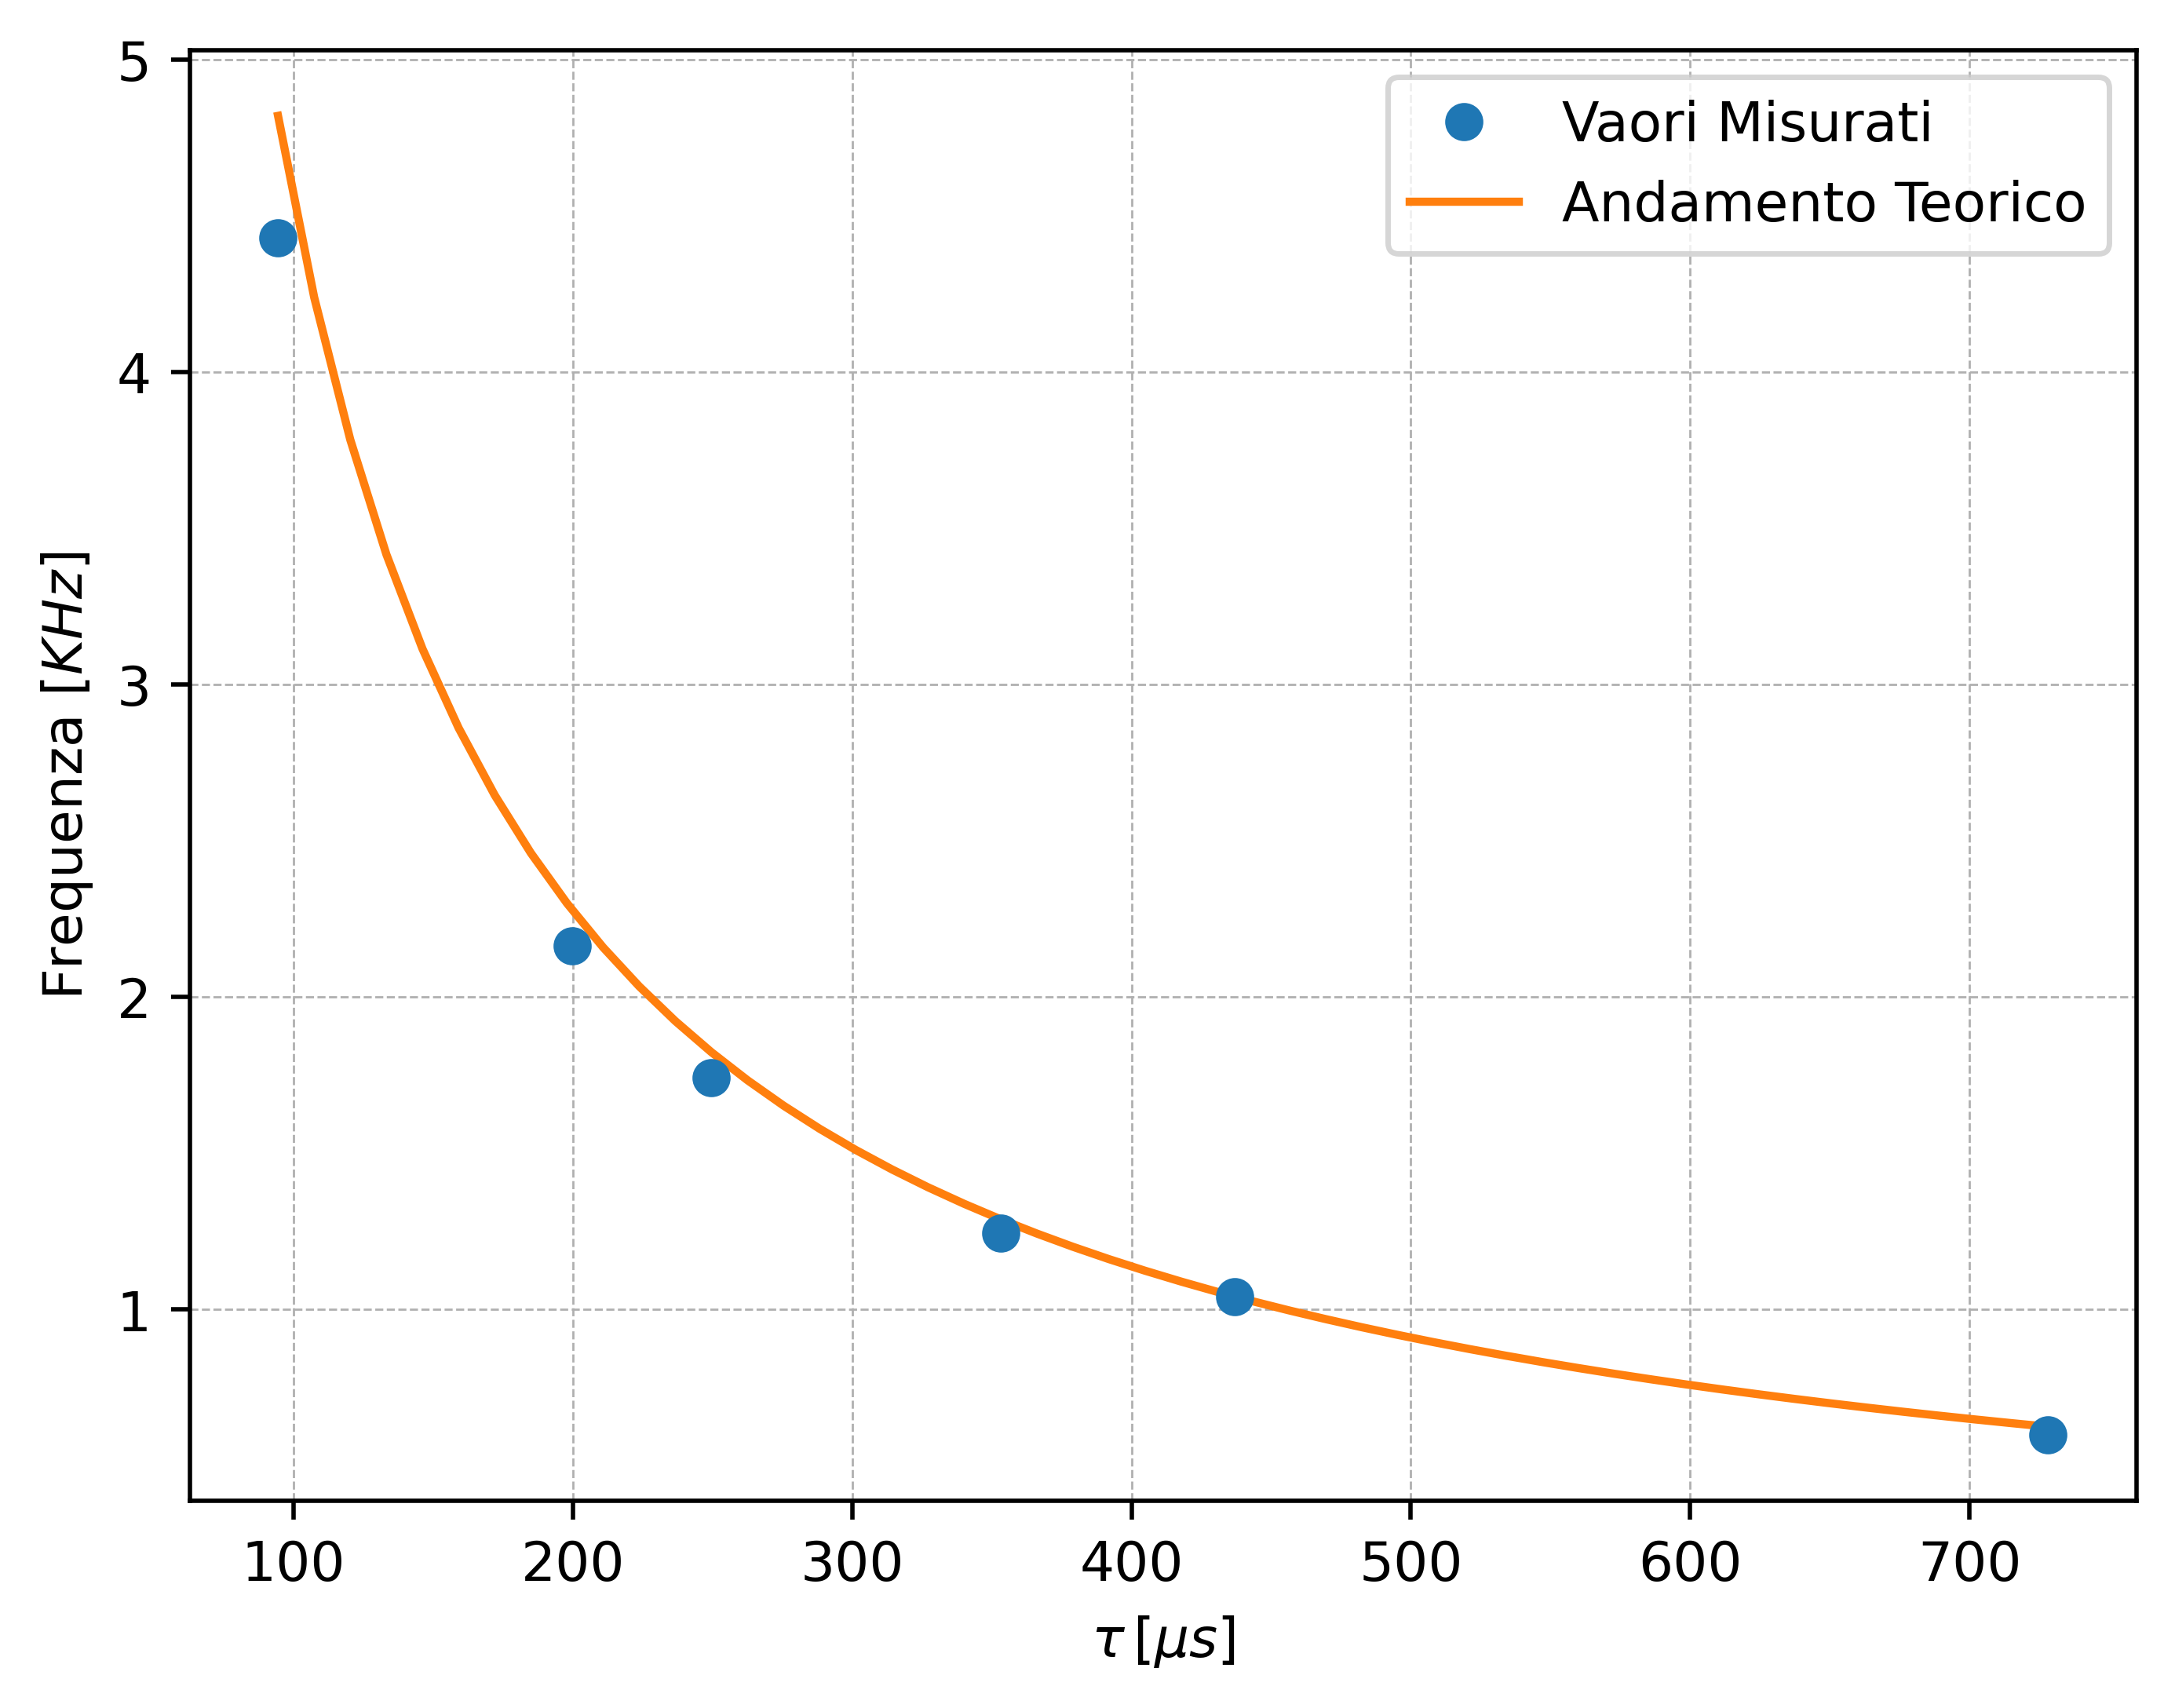
\includegraphics[width=0.6\linewidth]{immagini/ocillatore/freq_tau.png}
    \caption{Variazione della frequenza al variare della costante di tempo $\tau$.}
    \label{fig:ocillatore_freq_tau}
\end{figure}

In questo circuito si ottiene un duty cycle del 50 dovuto alla carica e scarica del condensatore sulla stessa resistenza. Di conseguenza se si volesse modificare questo aprametro si dovrebbe utilizzare un schema circuitale composto da due diodi opposti con resistenze R3 e R4 diverse.

\section*{Monostabile}
Il Monostabile è un circuito elettronico che riceve in ingresso un segnale e dà in uscita un impulso di durata ben definita. 
Inoltre, il fronte d'onda ascendente del segnale in uscita è sincronizzato con il fronte d'onda discendente del segnale in ingresso.

\begin{figure}[h]
    \centering
    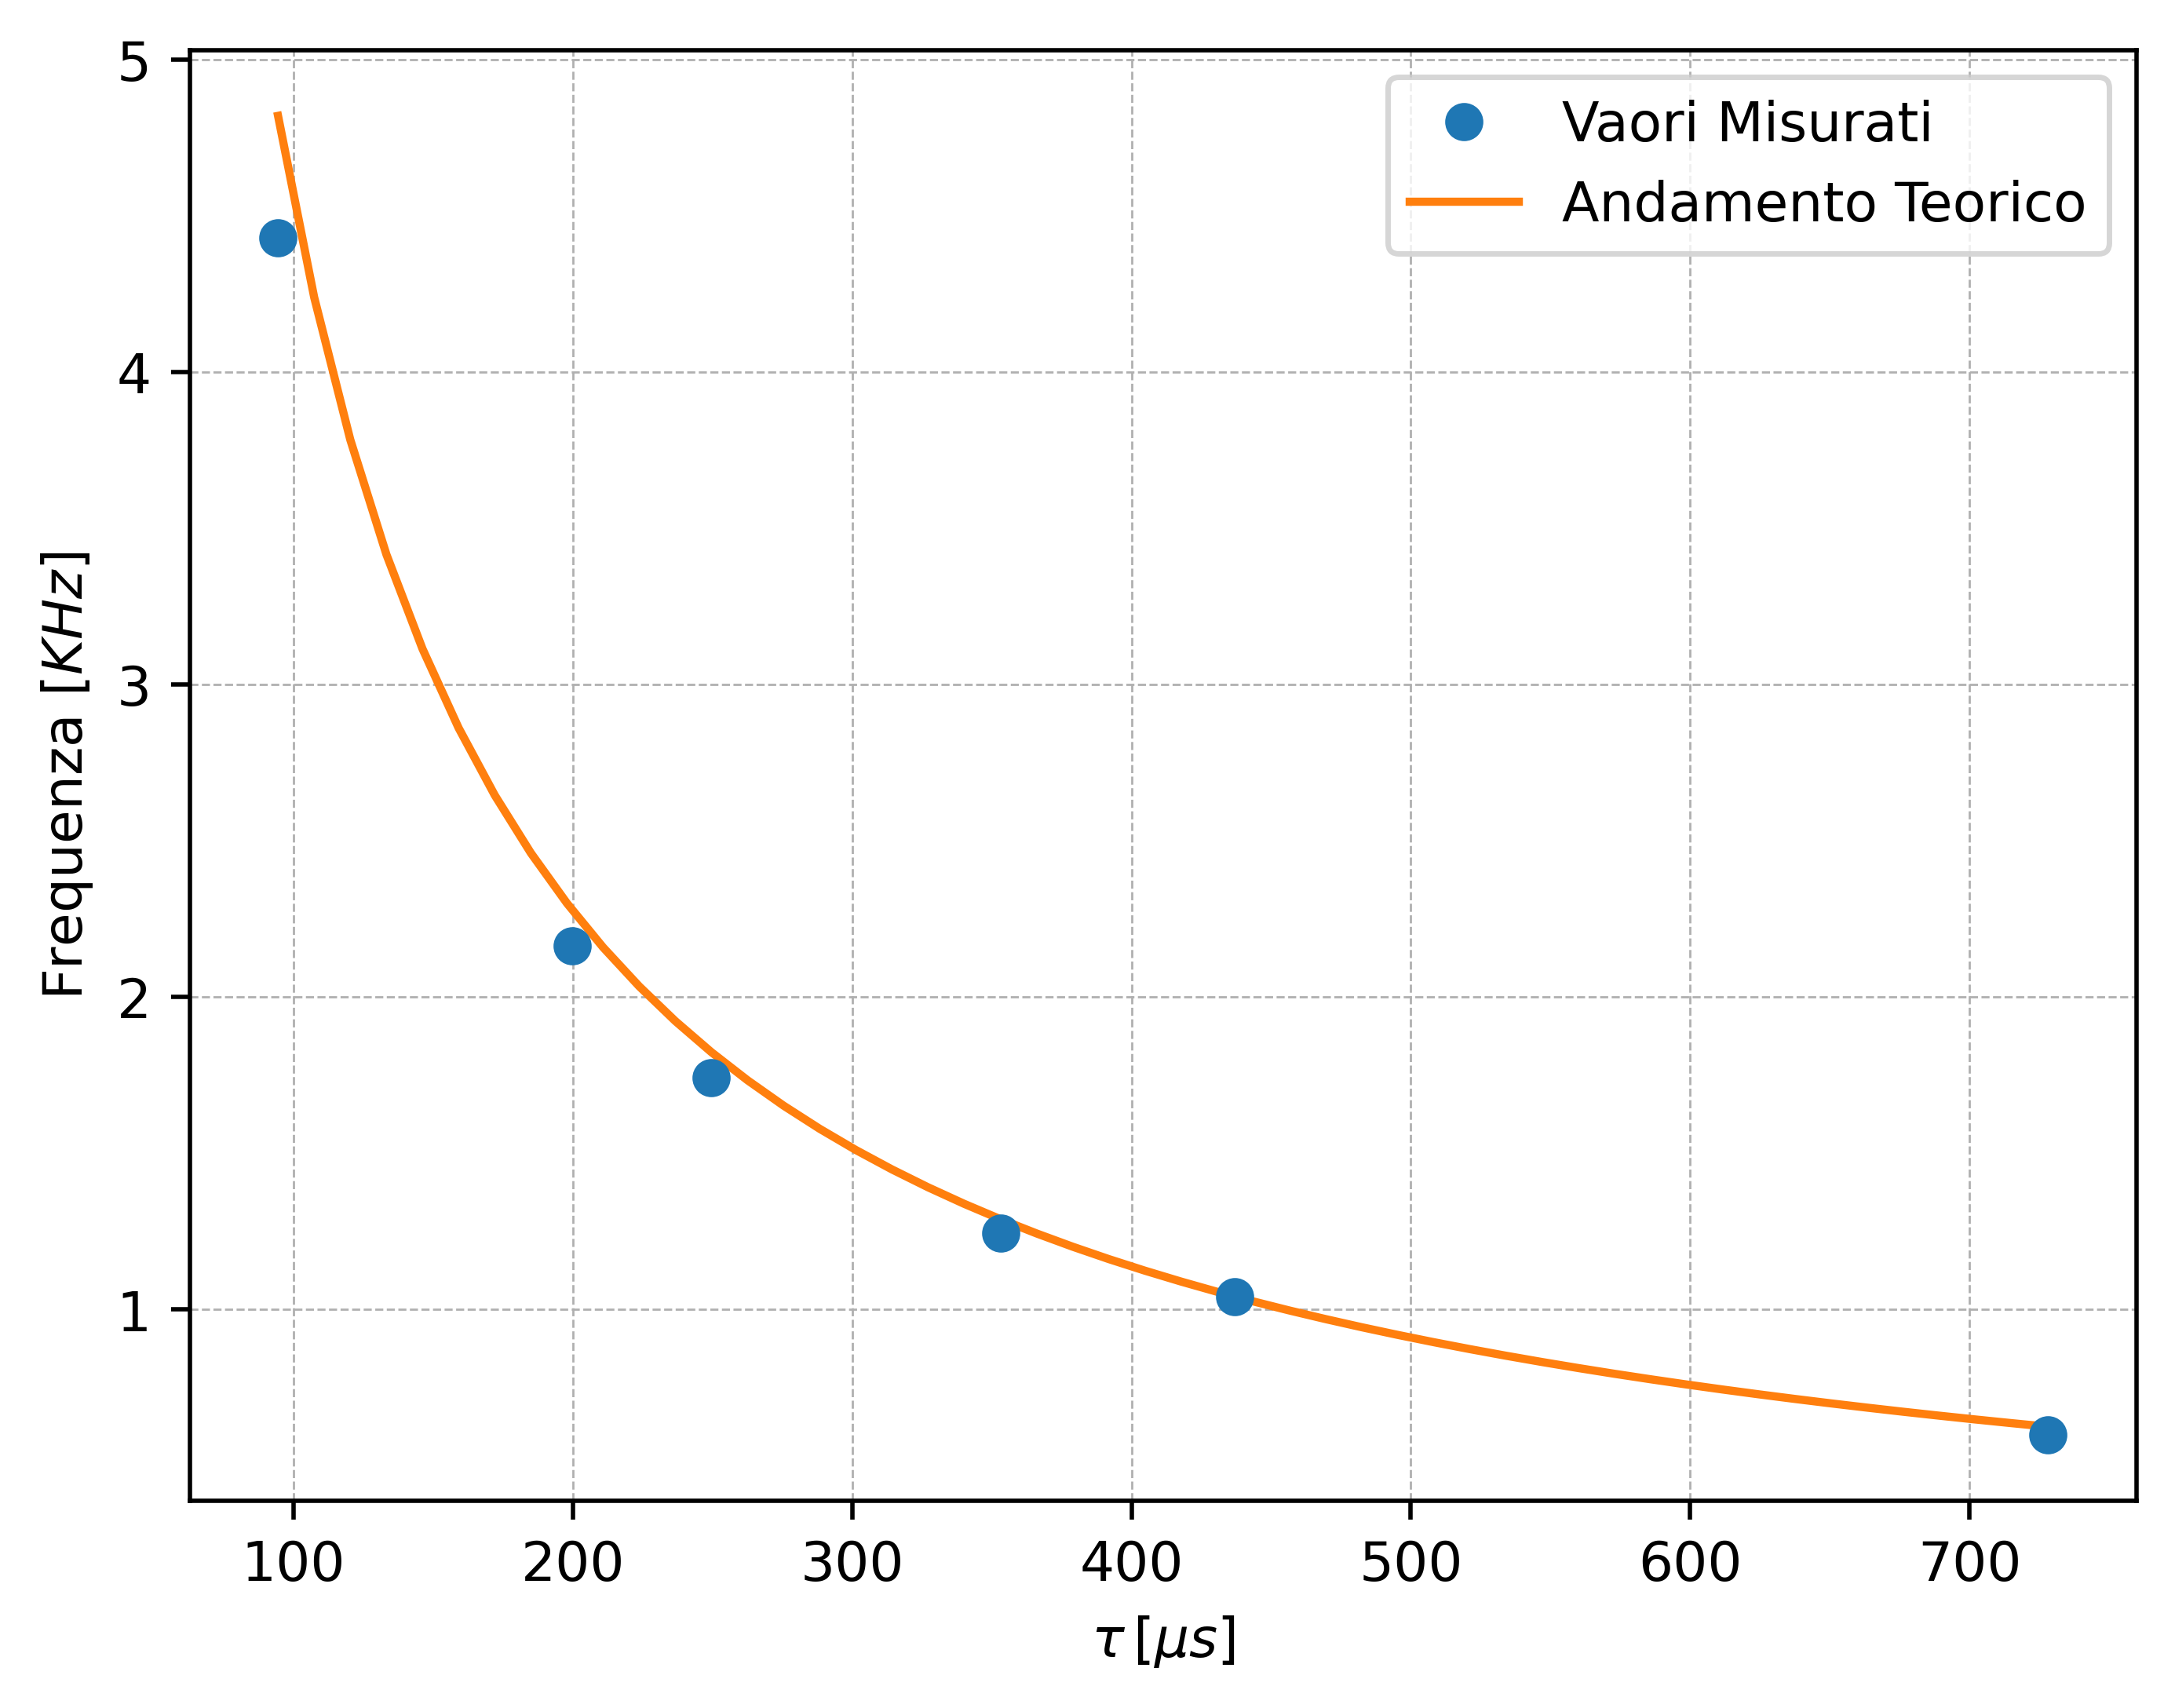
\includegraphics[width=0.6\linewidth]{immagini/ocillatore/freq_tau.png}
    \caption{Variazione della frequenza al variare della costante di tempo $\tau$.}
    % \label{fig:ocillatore_freq_tau}
\end{figure}

In una configurazione iniziale con diodo collegato in parallelo alla capacità, questo porta l'uscita ad essere costante al valore di accensione del diodo circa 0.7V a causa del fluire della corrente nel percorso a resistenza più bassa e quindi la capacità smette di caricarsi.

La presenza del derivatore (filtro passa-alto) permette di estrarre gli impulsi a delta di dirac da un segnale in ingresso e questo fa si che la soglia dinamica cambi.
In aggiunta, collegando un diodo al derivatore fa si che passino solo gli impulsi negativi e quindi che il segnale venga disaccoppiato dal resto del circuito.

La durata dell'impulso è definita dalla costante tau e dalle resistenze R1 e R2:
formule...

Tabella dati 
f=100hz
Vdd=10V
R=tre da 9khom e una resistenza variabile da 10.3kohm
C=70nF
CT=1nF


\end{document}

